\section{Results}
\subsection{Measurement for natural angular frequency}
    We calculate the angular frequency from Table \ref{data_omega} by the fomula
    \[
        \omega_0=\frac{2\pi}{T}.
    \]
    \begin{table}[H] \small
        \centering
        \begin{tabular}{|c|c|}
        \hline
            & $10T[s] \pm 0.001[s]$\\\hline
            1 & 15.481\\\hline
            2 & 15.480\\\hline
            3 & 15.496\\\hline
            4 & 15.481\\\hline
        \end{tabular}
        \caption{Measurement of ten periods}\label{data_omega}
    \end{table}

    Hence the average value of $10T$ should be calculated as
    \[
        \overline{10T}=\frac{1}{4}\sum_{i=1}^{4}(10T)_i=15.485 \pm 0.017 s, \quad u_{10T,r}=0.11\%.
    \]

    THe value of $\omega_0$ is
    \[
        \overline{\omega_0}=\frac{20\pi}{10T}=\frac{20\times3.1416}{15.485}=4.058\pm 0.004rad/s,\quad u_{\omega_0,r}=0.10\%.
    \]

\subsection{Measurement for damping coefficient}
    The damping coeffiecient can be calculated by the formula below.
    \[
        \beta=\frac{1}{5T}\ln\frac{\theta_i}{\theta_{i+5}}.
    \]
    \begin{table}[H] \small
        \centering
        \begin{tabular}{|c|c|c|c|c|}
        \hline
            \multicolumn{2}{|c}{Amplitude[$\degree$]$\pm$1[$\degree$]} & 
            \multicolumn{2}{|c|}{Amplitude[$\degree$]$\pm$1[$\degree$]} &
            $\ln(\theta_i/\theta_{i+5})$\\\hline
            $\theta_0$ & 89 & $\theta_5$ & 54 & 0.500\\\hline
            $\theta_1$ & 81 & $\theta_6$ & 49 & 0.503\\\hline
            $\theta_2$ & 73 & $\theta_7$ & 44 & 0.506\\\hline
            $\theta_3$ & 66 & $\theta_8$ & 40 & 0.501\\\hline
            $\theta_4$ & 60 & $\theta_9$ & 36 & 0.511\\\hline
            \multicolumn{4}{|c|}{The average value of $\ln(\theta_i/\theta_{i+5})$} & 0.504\\\hline
        \end{tabular}
        \caption{Measurement of the damping coefficient}\label{data_damping}
    \end{table}

    The expermental value of $\ln(\theta_i/\theta_{i+5})$ is shown below
    \[
        \ln(\theta_i/\theta_{i+5})=0.511\pm0.022 [no\ unit], \quad u_r=4\%
    \]

    Here, $T=15.561/10=1.5561\pm0.0001s$. Then we can easily obtain $\beta$ as well,
    \[
        \beta=\frac{1}{5\times1.5561}\times0.511=0.0657\pm 0.003s^{-1}, \quad u_{\beta,r}=4\%
    \]

\subsection{Measurement for $\theta_{st}$ vs. $\omega$ and $\varphi$ vs. $\omega$}
    To study the relation between $\varphi$ and $\omega/\omega_0$, we process the raw data and list them in Table \ref{data_phi2} and \ref{data_phi3}.
    \begin{figure}[H]
    \centering
    \begin{minipage}{0.4\textwidth}
        \begin{table}[H]
        \centering
            \begin{tabular}{|c|c|c|c|c|}
                \hline
                No. & $\omega/\omega_0[\ ]$ & $u_{\omega/\omega_0}[\ ]$ & $\varphi[\degree]$ & $u_{\varphi}[\degree]$\\\hline
                1 & 1.0416 & 0.0010 & -162 & 1\\\hline
                2 & 1.0296 & 0.0010 & -153 & 1\\\hline
                3 & 1.0187 & 0.0010 & -143 & 1\\\hline
                4 & 1.0110 & 0.0010 & -131 & 1\\\hline
                5 & 1.0075 & 0.0010 & -121 & 1\\\hline
                6 & 1.0050 & 0.0010 & -110 & 1\\\hline
                7 & 1.0032 & 0.0010 & -102 & 1\\\hline
                8 & 1.0018 & 0.0010 & -95 & 1\\\hline
                9 & 1.0011 & 0.0010 & -93 & 1\\\hline
                10 & 1.0006 & 0.0010 & -90 & 1\\\hline
                11 & 0.9998 & 0.0010 & -86 & 1\\\hline
                12 & 0.9980 & 0.0010 & -82 & 1\\\hline
                13 & 0.9965 & 0.0010 & -76 & 1\\\hline
                14 & 0.9943 & 0.0010 & -70 & 1\\\hline
                15 & 0.9915 & 0.0010 & -63 & 1\\\hline
                16 & 0.9892 & 0.0010 & -57 & 1\\\hline
                17 & 0.9870 & 0.0010 & -52 & 1\\\hline
                18 & 0.9860 & 0.0010 & -50 & 1\\\hline
                19 & 0.9843 & 0.0010 & -47 & 1\\\hline
                20 & 0.9812 & 0.0010 & -43 & 1\\\hline
                21 & 0.9772 & 0.0010 & -37 & 1\\\hline
                22 & 0.9712 & 0.0010 & -30 & 1\\\hline
                23 & 0.9640 & 0.0010 & -25 & 1\\\hline
            \end{tabular}
            \caption{$\varphi$ vs. $\omega/\omega_0$, Damping selection 2}\label{data_phi2}
        \end{table}
    \end{minipage}
    ~
    \begin{minipage}{0.4\textwidth}
        \begin{table}[H]
        \centering
            \begin{tabular}{|c|c|c|c|c|}
                \hline
                No. & $\omega/\omega_0[\ ]$ & $u_{\omega/\omega_0}[\ ]$ & $\varphi[\degree]$ & $u_{\varphi}[\degree]$\\\hline
                1 & 0.9624 & 0.0010 & -26 & 1\\\hline
                2 & 0.9669 & 0.0010 & -30 & 1\\\hline
                3 & 0.9715 & 0.0010 & -34 & 1\\\hline
                4 & 0.9771 & 0.0010 & -41 & 1\\\hline
                5 & 0.9818 & 0.0010 & -48 & 1\\\hline
                6 & 0.9868 & 0.0010 & -56 & 1\\\hline
                7 & 0.9925 & 0.0010 & -69 & 1\\\hline
                8 & 0.9954 & 0.0010 & -77 & 1\\\hline
                9 & 0.9971 & 0.0010 & -81 & 1\\\hline
                10 & 0.9976 & 0.0010 & -85 & 1\\\hline
                11 & 1.0004 & 0.0010 & -93 & 1\\\hline
                12 & 1.0022 & 0.0010 & -99 & 1\\\hline
                13 & 1.0039 & 0.0010 & -106 & 1\\\hline
                14 & 1.0056 & 0.0010 & -112 & 1\\\hline
                15 & 1.0068 & 0.0010 & -117 & 1\\\hline
                16 & 1.0083 & 0.0010 & -122 & 1\\\hline
                17 & 1.0107 & 0.0010 & -129 & 1\\\hline
                18 & 1.0132 & 0.0010 & -135 & 1\\\hline
                19 & 1.0158 & 0.0010 & -140 & 1\\\hline
                20 & 1.0191 & 0.0010 & -146 & 1\\\hline
                21 & 1.0221 & 0.0010 & -150 & 1\\\hline
                22 & 1.0290 & 0.0010 & -155 & 1\\\hline
                23 & 1.0367 & 0.0010 & -158 & 1\\\hline
            \end{tabular}
            \caption{$\varphi$ vs. $\omega/\omega_0$, Damping selection 3}\label{data_phi3}
        \end{table}
    \end{minipage}
    \end{figure}

    \begin{figure}[H]
    \centering
        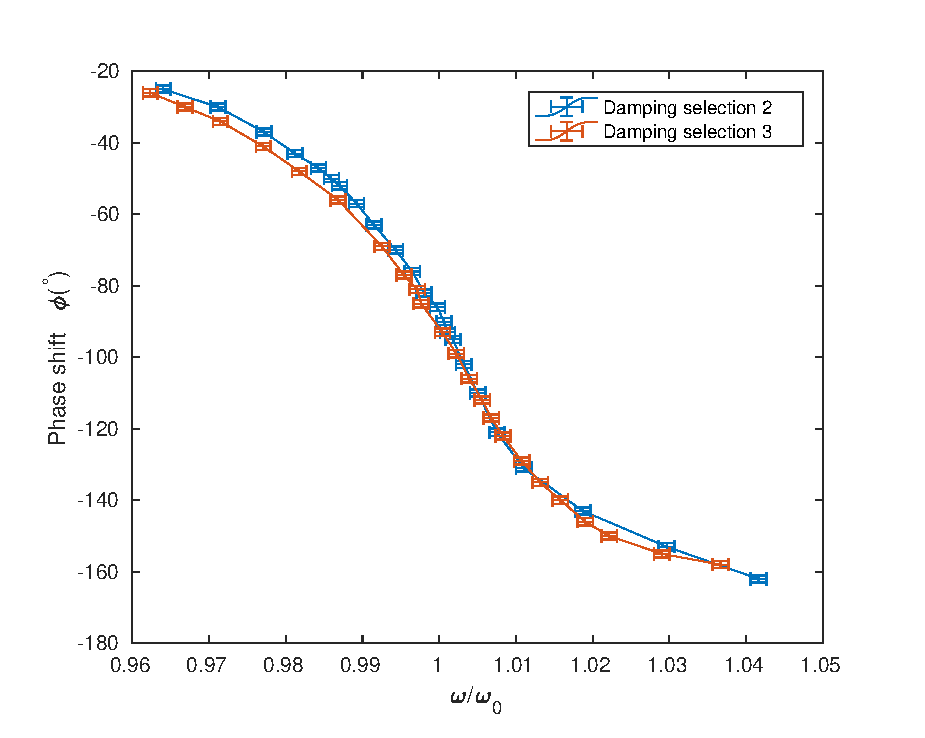
\includegraphics[width=0.65\textwidth]{images/phi}
        \caption{Phase shift $\varphi$ vs. $\omega/\omega_0$}\label{phi}
    \end{figure}


    To study the relation between $\theta_{st}$ and $\omega/\omega_0$, we process the raw data and list them in Table \ref{data_theta2} and \ref{data_theta3}.


    \begin{figure}[H]
    \centering
        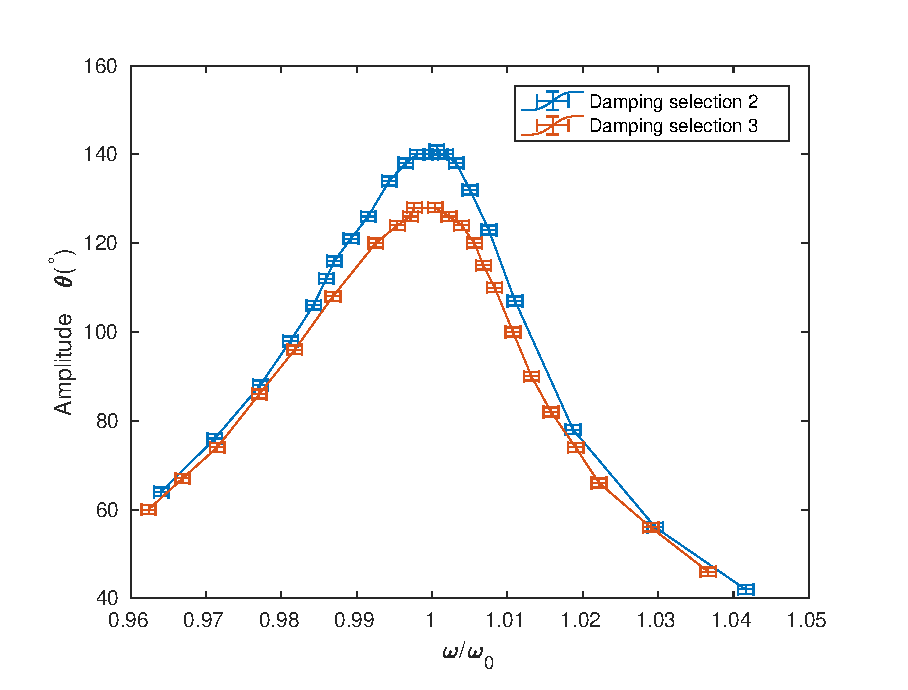
\includegraphics[width=0.65\textwidth]{images/theta}
        \caption{Amplitude $\theta_{st}$ vs. $\omega/\omega_0$}\label{theta}
    \end{figure}

    \begin{figure}[H]
    \centering
    \begin{minipage}{0.4\textwidth}
        \begin{table}[H]
        \centering
            \begin{tabular}{|c|c|c|c|c|}
                \hline
                No. & $\omega/\omega_0[\ ]$ & $u_{\omega/\omega_0}[\ ]$ & $\theta_{st}[\degree]$ & $u_{\theta_{st}}[\degree]$\\\hline
                1 & 1.0416 & 0.0010 & 42 & 1\\\hline
                2 & 1.0296 & 0.0010 & 56 & 1\\\hline
                3 & 1.0187 & 0.0010 & 78 & 1\\\hline
                4 & 1.0110 & 0.0010 & 107 & 1\\\hline
                5 & 1.0075 & 0.0010 & 123 & 1\\\hline
                6 & 1.0050 & 0.0010 & 132 & 1\\\hline
                7 & 1.0032 & 0.0010 & 138 & 1\\\hline
                8 & 1.0018 & 0.0010 & 140 & 1\\\hline
                9 & 1.0011 & 0.0010 & 140 & 1\\\hline
                10 & 1.0006 & 0.0010 & 141 & 1\\\hline
                11 & 0.9998 & 0.0010 & 140 & 1\\\hline
                12 & 0.9980 & 0.0010 & 140 & 1\\\hline
                13 & 0.9965 & 0.0010 & 138 & 1\\\hline
                14 & 0.9943 & 0.0010 & 134 & 1\\\hline
                15 & 0.9915 & 0.0010 & 126 & 1\\\hline
                16 & 0.9892 & 0.0010 & 121 & 1\\\hline
                17 & 0.9870 & 0.0010 & 116 & 1\\\hline
                18 & 0.9860 & 0.0010 & 112 & 1\\\hline
                19 & 0.9843 & 0.0010 & 106 & 1\\\hline
                20 & 0.9812 & 0.0010 & 98 & 1\\\hline
                21 & 0.9772 & 0.0010 & 88 & 1\\\hline
                22 & 0.9712 & 0.0010 & 76 & 1\\\hline
                23 & 0.9640 & 0.0010 & 64 & 1\\\hline
            \end{tabular}
            \caption{$\theta_{st}$ and $\omega/\omega_0$, Damping selection 2}\label{data_theta2}
        \end{table}
    \end{minipage}
    ~
    \begin{minipage}{0.4\textwidth}
        \begin{table}[H]
        \centering
            \begin{tabular}{|c|c|c|c|c|}
                \hline
                No. & $\omega/\omega_0[\ ]$ & $u_{\omega/\omega_0}[\ ]$ & $\theta_{st}[\degree]$ & $u_{\theta_{st}}[\degree]$\\\hline
                1 & 0.9624 & 0.0010 & 60 & 1\\\hline
                2 & 0.9669 & 0.0010 & 67 & 1\\\hline
                3 & 0.9715 & 0.0010 & 74 & 1\\\hline
                4 & 0.9771 & 0.0010 & 86 & 1\\\hline
                5 & 0.9818 & 0.0010 & 96 & 1\\\hline
                6 & 0.9868 & 0.0010 & 108 & 1\\\hline
                7 & 0.9925 & 0.0010 & 120 & 1\\\hline
                8 & 0.9954 & 0.0010 & 124 & 1\\\hline
                9 & 0.9971 & 0.0010 & 126 & 1\\\hline
                10 & 0.9976 & 0.0010 & 128 & 1\\\hline
                11 & 1.0004 & 0.0010 & 128 & 1\\\hline
                12 & 1.0022 & 0.0010 & 126 & 1\\\hline
                13 & 1.0039 & 0.0010 & 124 & 1\\\hline
                14 & 1.0056 & 0.0010 & 120 & 1\\\hline
                15 & 1.0068 & 0.0010 & 115 & 1\\\hline
                16 & 1.0083 & 0.0010 & 110 & 1\\\hline
                17 & 1.0107 & 0.0010 & 100 & 1\\\hline
                18 & 1.0132 & 0.0010 & 90 & 1\\\hline
                19 & 1.0158 & 0.0010 & 82 & 1\\\hline
                20 & 1.0191 & 0.0010 & 74 & 1\\\hline
                21 & 1.0221 & 0.0010 & 66 & 1\\\hline
                22 & 1.0290 & 0.0010 & 56 & 1\\\hline
                23 & 1.0367 & 0.0010 & 46 & 1\\\hline
            \end{tabular}
            \caption{$\theta_{st}$ and $\omega/\omega_0$, Damping selection 3}\label{data_theta3}
        \end{table}
    \end{minipage}
    \end{figure}
